

\begin{scifitablebox}[screenbox, title=\textcolor{PanelGlow}{Vehicle Stats}]
\begin{itemize}
    \item \textbf{Armor Class (AC)} \textit{- Standard}
    \item \textbf{Hull Points (HP)} \textit{- Vehicle health}
    \item \textbf{Shield Points} \textit{- Absorb damage before hull. Can only regenerate in combat via the Restore action}
    \item \textbf{Speed} \textit{- Number of spaces the vehicle can move per turn (combat scale)}
    \item \textbf{Range} \textit{- Distance traveled in a 24-hour period}
    \item \textbf{Minimum Crew} \textit{- Required crew to operate normally (Operating below minimum may impose disadvantage)}
    \item \textbf{Crew Capacity} \textit{- Total number of occupants (crew + passengers)}
    \item \textbf{Cargo Capacity} \textit{- Measured in Megagrams (Mg). 1 Mg = 1,000 kg (~2,200 lbs)}
    \item \textbf{Systems} \textit{- Individual ship functions.}
    \item \textbf{Weapons} \textit{- Weapons on the vehicle. (roll then multiply)}
    \item \textbf{Size} \textit{- Size of vehicle, has multiple categories, and special categories for starships.}
    \item \textbf{Cost} \textit{- Listed cost = market value. Military vehicles are not normally available for purchase}
\end{itemize}
\end{scifitablebox}


\begin{scifitablebox}[screenbox,title=\textcolor{PanelGlow}{Vehicle Systems}]
\begin{itemize}
\item Systems are functional stations within a vehicle where specific actions are performed.
\item Crew must be at the relevant system to use its abilities.
\end{itemize}
\begin{itemize}
\item \textbf{Helm} \textit{- Pilot station.}
\item \textbf{Navigation} \textit{- Required for plotting FTL jumps no matter method.}
\item \textbf{Weapons} \textit{- Required for \underline{Attack} action}
\item \textbf{EWS (Electronic Warfare Suite)} \textit{- Protects against and enables hacking}
\item \textbf{SSC (Sensors, Scanners, Communications)} \textit{- Scan planets and objects. Communication with ships/planets.}
\item \textbf{Drive (Engineering)} \textit{Can be used for power redirection.}
\end{itemize}

\textbf{Additional Systems \& Upgrades}
\begin{itemize}
\item Ships may include extra systems (quarters, labs, workshops, etc.)
\item Installing/upgrading systems:
\begin{itemize}
\item Takes 8 hours of uninterrupted work
\item Can hire help or perform yourself
\end{itemize}
\item Replacing a broken system costs 300,000 or the price of the system in the ship upgrades table, whichever is lower.
\end{itemize}
\end{scifitablebox}

  \begin{scifitablebox}[screenbox,title=\textcolor{PanelGlow}{Disgruntled Crew}]
Each month you will need to pay 150 x number of crew x 30 credits, or 1d6 members of crew become disgruntled.\\
\textbf{Dealing with Disgruntled Crew:}
\begin{itemize}
    \item Fire the disgruntled crew member. (They will disappear at next habital station)
    \item Throw the crew member out an airlock. 1d6 crew members become disgruntled in response.
    \item Provide bonus pay equal to one week's salary (150 x Crew size x 7)
    \item Provide an extended stay at a port (2 long rests worth)
\end{itemize}
\end{scifitablebox}
\newcolumn
\longeffecttable{Months without maintenance}
  {Months}
  {Effect}
  {
    1 & Any checks made at the system are made at disadvantage and any downtime activities completed with the system take twice as long. \\
    2 & Roll a d20. On a 5 or less, the system breaks and cannot be used in any way. It must be replaced. \\
    3 & Roll a d20. On a 10 or less, the system breaks and cannot be used in any way. It must be replaced. \\
    4 & Roll a d20. On a 15 or less, the system breaks and cannot be used in any way. It must be replaced. \\
    5 & The system breaks and cannot be used in any way. It must be replaced.
  }
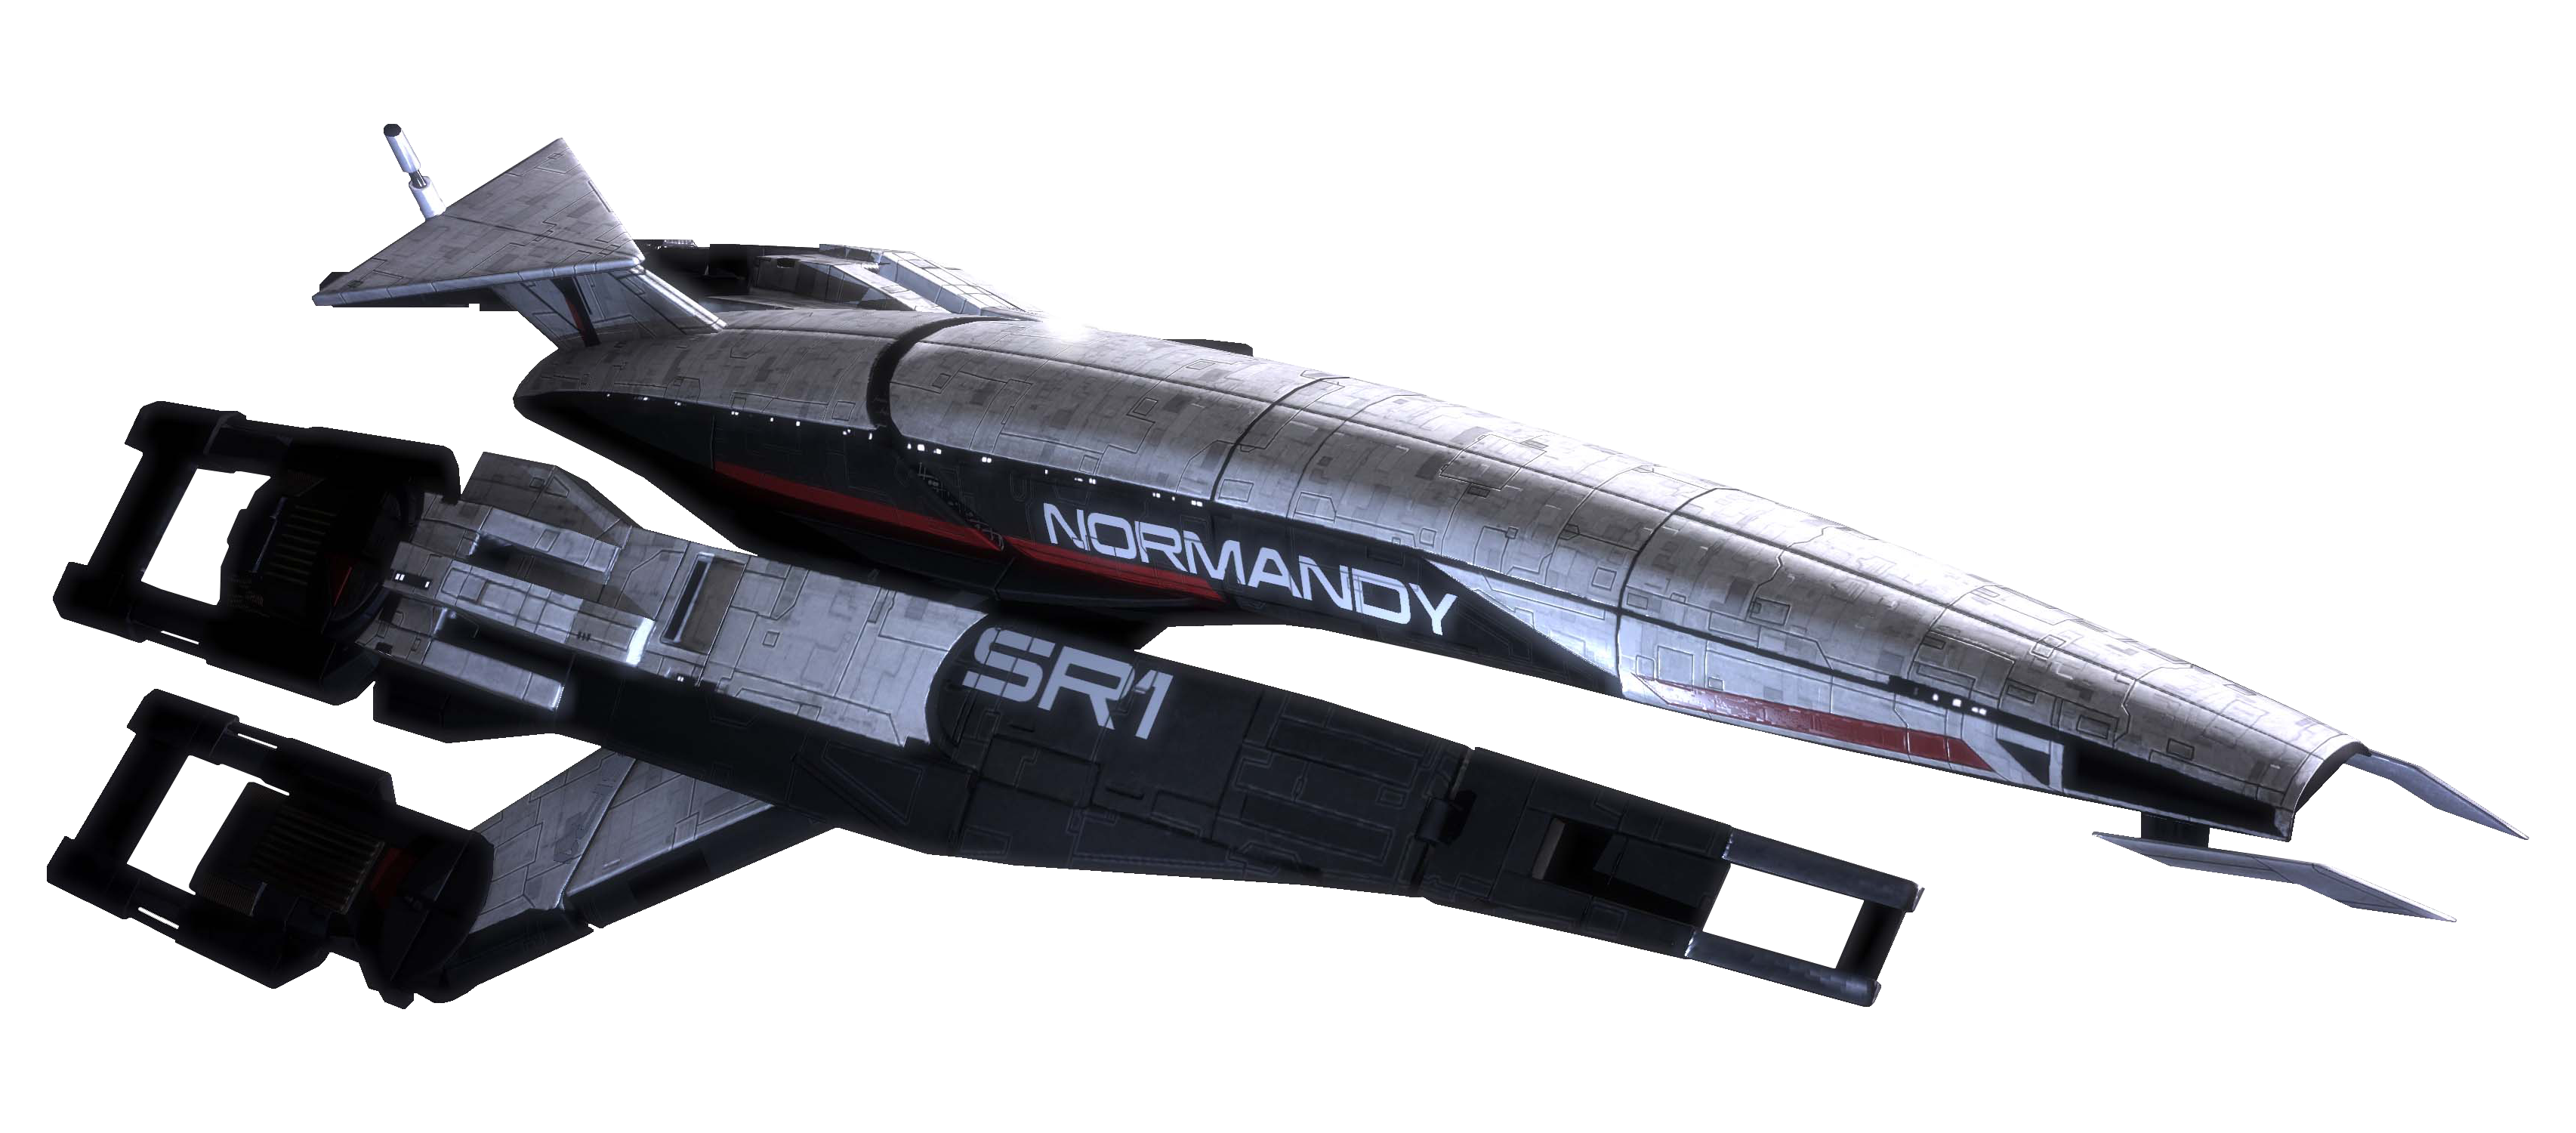
\includegraphics[width=\linewidth]{assets/Normandy.png}
\newpage
\longeffecttable{Disgruntled Crew}
  {d20 + crew}
  {Effect}
  {
    1-5 & Nothing happens.\\
    6-8 & A fight breaks out between two crew members. Another member of your crew becomes disgruntled.\\
    9-11 & One of your disgruntled crew quits the next time you’re at port.\\
    12-13 & A crew member starts an private email chain that infuriates the other crew. Two additional crew become disgruntled.\\
    14-15 & All of your disgruntled crew quit the next time you’re at port.\\
    16-17 & A crew member forgets to service their system. You must pay 3,000 credits before you can use it again. (If this is the Drive, you ship cannot move between systems)\\
    18-19& A crew member sabotages their system. You must pay 20,000 credits before you can use it again. (If this is the Drive, you ship cannot move between systems)\\
    20+& The crew mutinies. They all become hostile and attack your party.\\
  }